% =================================================================================================
% Roman's per-exposure astrometric error model: what it is, where it lives in the code, and how it
% enters the astrometric Fisher matrix.  A model note, not a production-run report, so the
% template's run / yield / weighting sections do not apply and were dropped.
%
% Code state described: branch joint-fisher-refactor, HEAD 36c7fd2 (2026-10-03).
% Line numbers below are for that commit; the function and constant NAMES are the stable handles.
% Provenance in DEVIATIONS.md: 29 (Step H4, the model), 71 (per-coordinate sigma, free reference
% position, W/N/P variants), 72 (AB -> Vega), 74 (blended centroid), 75 (finite-difference steps).
%
% Build:  cd Report/roman_astrometry && latexmk -pdf roman_astrometry_report.tex
% =================================================================================================
\documentclass[english,10pt,a4paper]{article}
\usepackage[T1]{fontenc}
\usepackage[margin=2.4cm]{geometry}
\usepackage{graphicx}
\usepackage{mathtools}
\usepackage{amssymb}
\usepackage{booktabs}
\usepackage{tabularx}
\usepackage{xcolor}
\usepackage[colorlinks=true,allcolors=blue]{hyperref}
\usepackage{caption}
\usepackage[authoryear,round]{natbib}
\usepackage[section]{placeins}
\usepackage{pgfplots}
\pgfplotsset{compat=1.18}

\newcommand{\tE}{t_{\rm E}}
\newcommand{\piE}{\pi_{\rm E}}
\newcommand{\tetE}{\theta_{\rm E}}
\newcommand{\Ml}{M_{\rm L}}
\newcommand{\code}[1]{\texttt{#1}}
\newcommand{\TODO}[1]{\textcolor{red}{\textbf{[TODO: #1]}}\typeout{TODO: #1}}

\title{The Roman astrometric error model}
\author{Ali Salehi}
\date{\today}

\begin{document}
\maketitle

\begin{abstract}
Each Roman F146 exposure gets a per-coordinate astrometric error $\sigma_{\rm ast}$ that depends
only on the epoch's blended, magnified F146 magnitude. It is a three-branch curve: a 1.1\,mas
centroiding floor (1\% of a 110\,mas pixel) down to $m_{\rm Vega}=20.62$, then a rise through
10\,mas at $m_{\rm Vega}=23.5$, then a background-dominated rise of 0.4\,dex per magnitude
\citep{Sanderson2019WFIRSTastrometry,Lam2026BHbinaries}. The error is \emph{per exposure}
(one 66\,s exposure every 12.1\,min), not the 0.1\,mas daily-binned figure. Over the magnitudes
Roman records, 14.8--25.45 (AB), it spans 1.1--23.3\,mas. In the astrometric Fisher matrix
each coordinate of each exposure is weighted by $1/\sigma_{\rm ast}^2$, and the source's reference
position is marginalised over. Whether the floor averages down is not known, so every event
carries three forecasts: white noise (W, the literature's assumption and the main output columns),
nominal (N) and pessimistic (P). N and P add a per-day correlated error and more free offsets.
This note gives each piece with its exact location in the code.
\end{abstract}

% -------------------------------------------------------------------------------------------------
\section{The per-exposure error}
\label{sec:model}

The function is \code{errRomanA(double magF146AB)}, defined in \code{helper.cpp} (line 256) and
declared in \code{Bulge.h} (line 1401). It takes the epoch's F146 AB magnitude $m$ and returns
$\sigma_{\rm ast}$ in mas, the 1D precision in $x$ \emph{or} $y$ of one exposure. Its
literature anchors are Vega magnitudes, so it converts first:
\begin{equation}
m_{\rm V} = m - \Delta_{\rm AB-V}, \qquad \Delta_{\rm AB-V} = 1.0324 ,
\end{equation}
and then evaluates
\begin{equation}
\sigma_{\rm ast}(m_{\rm V}) =
\begin{cases}
1.1\ {\rm mas}, & m_{\rm V} \le 20.62,\\[2pt]
1.1 \times 10^{\,0.33285\,(m_{\rm V}-20.62)}\ {\rm mas}, & 20.62 < m_{\rm V} \le 23.5,\\[2pt]
10.0 \times 10^{\,0.4\,(m_{\rm V}-23.5)}\ {\rm mas}, & m_{\rm V} > 23.5,
\end{cases}
\label{eq:sigast}
\end{equation}
clamped from below at 1.1\,mas, with \code{CHECK}s that the result is finite and at least the floor.
The branches meet without jumps: the middle slope is
$\log_{10}(10/1.1)/(23.5-20.62)=0.33285$\,dex\,mag$^{-1}$, set by the two published anchors.
It is not a free choice. It falls between source-dominated photon noise (0.2) and pure background
domination (0.4) because the transition is already under way across that range. The function reads no data file and needs no
instrument struct. Table~\ref{tab:const} lists every constant, and Figure~\ref{fig:curve} plots the curve.

\begin{table}[h]
\centering
\caption{Constants of Eq.~\eqref{eq:sigast}, all in \code{Bulge.h}.}
\label{tab:const}
\small
\begin{tabularx}{\textwidth}{@{}l r l X@{}}
\toprule
constant & value & line & source / meaning \\
\midrule
\code{F146\_AB\_MINUS\_VEGA}  & 1.0324     & 351 & AB magnitude of Vega (CALSPEC \code{alpha\_lyr\_stis\_011}) through STScI's F146 effective area \code{Roman\_effarea\_v8\_SCA01\_20240301}, synphot (Deviation 72) \\
\code{ROMAN\_PIX\_MAS}        & 110 mas    & 352 & WFI pixel, 0.11$''$ \citep{Lam2026BHbinaries} \\
\code{ROMAN\_AST\_FLOOR}      & 1.1 mas    & 353 & $0.01\times$ pixel: 1\% centroiding \citep[§1.1]{Sanderson2019WFIRSTastrometry}; \citep[Fig.~5]{Lam2026BHbinaries} \\
\code{ROMAN\_AST\_MFLR}       & 20.62      & 354 & F146$_{\rm Vega}$ below which the floor dominates \citep{Lam2026BHbinaries} \\
\code{ROMAN\_AST\_MBKG}       & 23.5       & 355 & F146$_{\rm Vega}$ where the background takes over \citep{Lam2026BHbinaries} \\
\code{ROMAN\_AST\_SBKG}       & 10.0 mas   & 356 & $\sigma_{\rm ast}$ at \code{ROMAN\_AST\_MBKG} \citep{Lam2026BHbinaries} \\
\code{ROMAN\_AST\_SLOPE\_SRC} & 0.33285    & 363 & slope joining the two anchors (derived, above) \\
\code{ROMAN\_AST\_SLOPE\_BKG} & 0.4        & 364 & background-dominated, SNR $\propto$ counts \\
\bottomrule
\end{tabularx}
\end{table}

\begin{figure}[h]
\centering
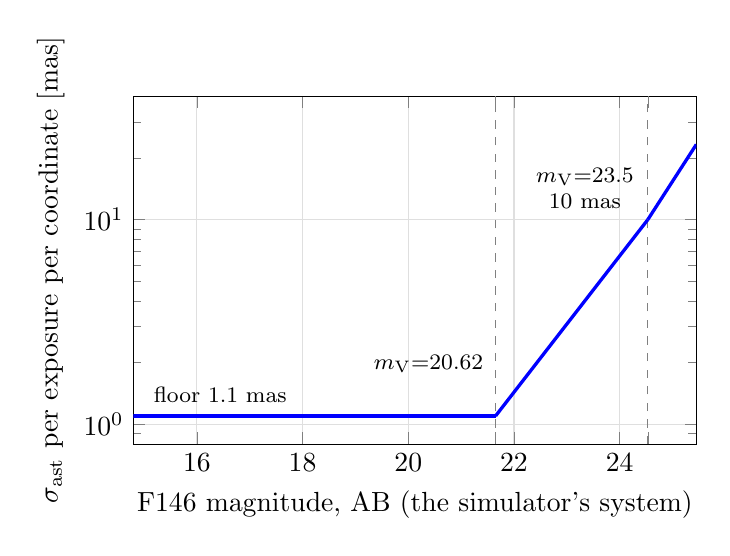
\begin{tikzpicture}
\begin{axis}[
  width=0.72\textwidth, height=6cm,
  xlabel={F146 magnitude, AB (the simulator's system)},
  ylabel={$\sigma_{\rm ast}$ per exposure per coordinate [mas]},
  ymode=log, xmin=14.8, xmax=25.45, ymin=0.8, ymax=40,
  grid=major, grid style={gray!25},
  extra x ticks={21.6524,24.5324}, extra x tick labels={}, extra x tick style={grid style={dashed,gray}},
]
\addplot[very thick, blue, domain=14.8:21.6524, samples=2] {1.1};
\addplot[very thick, blue, domain=21.6524:24.5324, samples=60] {1.1*10^(0.33285*(x-1.0324-20.62))};
\addplot[very thick, blue, domain=24.5324:25.45, samples=30] {10*10^(0.4*(x-1.0324-23.5))};
\node[anchor=south west, font=\footnotesize] at (axis cs:15.0,1.15) {floor 1.1 mas};
\node[anchor=south east, font=\footnotesize] at (axis cs:21.6,1.6) {$m_{\rm V}{=}20.62$};
\node[anchor=north east, font=\footnotesize, align=center] at (axis cs:24.45,20) {$m_{\rm V}{=}23.5$\\10 mas};
\end{axis}
\end{tikzpicture}
\caption{Eq.~\eqref{eq:sigast} on the simulator's AB scale. The plotted range is Roman's recording
window: saturation \code{ROMAN\_SATU\_AB} $=14.8$ to the single-exposure $5\sigma$ depth
\code{ROMAN\_DEPTH5\_AB} $=25.45$ (\code{Bulge.h} lines 193--194). Dashed lines mark the two
anchors, at AB 21.65 and 24.53.}
\label{fig:curve}
\end{figure}

\paragraph{Per exposure, not per day.}
Both sources also quote 0.1\,mas, but that is the precision after binning $\sim$100 exposures in a
day. One row of \code{Baseline/RomanBaseline.dat} is one exposure. The file has 302{,}406 rows,
50{,}401 per field for 6 fields, with a median spacing of 0.008403\,d $=12.1$\,min. Each row
therefore gets the 1.1\,mas per-exposure value. Using 0.1\,mas would overstate Roman's astrometry
tenfold (DEVIATIONS 29.1).

\paragraph{Per coordinate.}
$\sigma_{\rm ast}$ is the 1D error, as both sources define it \citep[fn.~14]{Lam2026BHbinaries}.
Each coordinate's variance is therefore $\sigma_{\rm ast}^2$, not $2\sigma_{\rm ast}^2$. The code
used the doubled variance until Deviation 71.

% -------------------------------------------------------------------------------------------------
\section{Where the error is computed and stored}
\label{sec:flow}

The error is evaluated once per recorded Roman epoch in the Roman branch of the light-curve time
loop in \code{main()} (\code{Bulge\_LSST.cpp}). Table~\ref{tab:flow} traces the path.

\begin{table}[h]
\centering
\caption{The path of one Roman exposure's astrometric error. Line numbers are for
\code{Bulge\_LSST.cpp} at commit \code{36c7fd2}.}
\label{tab:flow}
\small
\begin{tabularx}{\textwidth}{@{}l X@{}}
\toprule
where & what happens \\
\midrule
l.~962 (reader) & \code{Baseline/RomanBaseline.dat} is read into the \code{roman} struct: columns \code{ID RA Dec l b time sig5 field layout}. \code{time} sets the epoch and \code{layout} sets the roll (0/1). \\
l.~2162 & \code{magni[fiR]} $= m_{\rm bs} - 2.5\log_{10}(A\,f_b + 1 - f_b)$: the F146 AB magnitude of the \emph{whole blend} at this epoch, magnified. $m_{\rm bs}$ and $f_b$ are Roman's (telescope index 1) and include a luminous lens's light (Deviation 74). \\
l.~2167 & Gate: the epoch is recorded only if $14.8 \le$ \code{magni[fiR]} $\le 25.45$. \\
l.~2182 & \code{errsR = errRomanA(magni[fiR]);} \\
l.~2187--2196 & \code{errsR} also sets the image-resolution counts \code{nres5\_R}, \code{nres20\_R} (separation $\ge 5$ or $20\,\sigma_{\rm ast}$; \code{RESOLVE\_D\_*}, \code{Bulge.h} l.~478--479). \\
l.~2198--2205 & Noise draws \code{silR}, \code{sil2R} $=$ \code{RandN(errsR, 3.0)} (Gaussian truncated at $3\sigma$) feed the astrometric $\chi^2$ diagnostics \code{chi*a\_R} (the \code{dchiA*} columns). They are \emph{not} the detection test and do not enter the Fisher matrix. \\
l.~2229--2234 & Stored per datum: \code{l->erra[ndw] = errsR}, \code{l->tele[ndw] = 1} (Roman), \code{l->rseas[ndw] = sched.seasonOf(time)} (\code{helper.cpp} l.~830), \code{l->rroll[ndw] = layout}. Fields in \code{struct lens}, \code{Bulge.h} l.~798--801. \\
l.~3314 & \code{FisherM(...)} reads \code{l.erra[]} for every epoch (Section~\ref{sec:fisher}). \\
\bottomrule
\end{tabularx}
\end{table}

Because the input is the blended, magnified magnitude, $\sigma_{\rm ast}$ changes during the event.
It falls as the source brightens toward the peak and reaches the 1.1\,mas floor wherever the blend
is brighter than AB 21.65. The modelled position itself is the flux-weighted centroid of the
lensed source, the lens's own light and unresolved neighbours (\code{lightcurve()}, l.~4101--4102;
Deviation 74). The \emph{error} depends only on the total magnitude.

% -------------------------------------------------------------------------------------------------
\section{How it enters the astrometric Fisher matrix}
\label{sec:fisher}

The astrometric parameters are $\boldsymbol p=(\tetE,\mu_{s1},\mu_{s2},\piE)$, with $N_y=4$.
For each epoch $i$, \code{FisherM} computes the derivatives of both centroid coordinates,
$d^{x}_{ij}=\partial x_i/\partial p_j$ and $d^{y}_{ij}$. It uses central differences with steps
\code{co.Delta2[j]} $\approx 0.25\,p_j$ (l.~3688--3691; step sizes from the M3 sweep, Deviation 75),
and each epoch is evaluated from the observer that produced it (Earth or L2). The weight is
\begin{equation}
w_i = 1/\sigma_{{\rm ast},i}^2 \qquad\text{per coordinate} \qquad (\text{l.~3766}).
\end{equation}

\paragraph{Accumulation (l.~3710--3776).}
Rubin epochs go into one white block. Roman epochs go into \emph{day blocks}
$k=\lfloor t_i\rfloor$, each tagged with its season and roll. Every block keeps
$S_w=\sum w_i$, $\boldsymbol S^{c}_{wd}=\sum w_i\,\boldsymbol d^{c}_i$ and
$\mathsf S^{c}_{wdd}=\sum w_i\,\boldsymbol d^{c}_i\boldsymbol d^{c\,T}_i$ for $c\in\{x,y\}$
(\code{struct AstSums}).

\paragraph{A per-day correlated error (\code{Group::fold}, l.~3784).}
In the N and P variants, every Roman exposure of a day also shares one error of size $\sigma_c$
per coordinate. Adding $\sigma_c^2$ to every element of a day's covariance has an exact
Sherman--Morrison inverse, so each block enters as
\begin{align}
\mathsf F_k &= \sum_{c}\Big[\mathsf S^{c}_{wdd} - \frac{\sigma_c^2\,\boldsymbol S^{c}_{wd}\boldsymbol S^{c\,T}_{wd}}{1+\sigma_c^2 S_w}\Big], &
\boldsymbol b^{c}_k &= \frac{\boldsymbol S^{c}_{wd}}{1+\sigma_c^2 S_w}, &
c_k &= \frac{S_w}{1+\sigma_c^2 S_w}.
\end{align}
For $\sigma_c=0$ this reduces to plain white noise.

\paragraph{A free reference position (\code{Group::marginaliseInto}, l.~3794).}
A real astrometric fit solves for the source's position offset
\citep{Lam2026BHbinaries,McKinnon2026RomanGaia}. Without that offset, the model's constant
$-u_0\tetE\sin\xi$ term would let every exposure measure $\tetE$ from the absolute position.
Each \emph{frame group} $g$ therefore gets a free $(x_0,y_0)$, which is marginalised in closed form:
\begin{equation}
\mathsf F_g = \sum_{k\in g}\mathsf F_k \;-\; \sum_{c\in\{x,y\}}
\frac{\big(\sum_{k\in g}\boldsymbol b^{c}_k\big)\big(\sum_{k\in g}\boldsymbol b^{c}_k\big)^{T}}{\sum_{k\in g}c_k}.
\end{equation}
Roman's matrix is $\mathsf F_R=\sum_g\mathsf F_g$. Rubin's, $\mathsf F_L$, is one group with
$\sigma_c=0$. The joint matrix is exactly $\mathsf F_L+\mathsf F_R$ (l.~3802--3815), so
$\sigma_{\rm joint}\le\sigma_{\rm single}$ holds by construction.

\begin{table}[h]
\centering
\caption{The three noise variants (\code{enum AstroVariant} and \code{AST\_SIGC}, \code{Bulge.h}
l.~393--397). Rubin is white with one offset in all three.}
\label{tab:variants}
\small
\begin{tabularx}{\textwidth}{@{}l l l X@{}}
\toprule
variant & $\sigma_c$ per Roman day & Roman frame groups & rationale \\
\midrule
W (white)       & 0             & 1 (whole mission)        & The literature's assumption: the floor is white, which sub-pixel dithering justifies \citep{Lam2026BHbinaries,Sanderson2019WFIRSTastrometry}. \textbf{Main output columns.} \\
N (nominal)     & 0.3 mas       & 2 (one per roll)         & Distortion residuals at a few $\times0.1\%$ of a pixel (Bellini 2024, via \citealt{Lam2026BHbinaries}). Crowding biases flip with the PSF orientation. \\
P (pessimistic) & 1.1 mas       & one per season ($\le16$) & The whole floor is shared within a day and averages down only across days. Each season has its own frame. \\
\bottomrule
\end{tabularx}
\end{table}

\paragraph{Inversion and output.}
W fills \code{co.inputB[q]} for $q\in\{$\code{SJOINT}, \code{SRUBIN}, \code{SROMAN}$\}$. It is
inverted by \code{invert\_matrix(co, 1, q)} if that partition has at least $N_y$ astrometric epochs
(l.~3823), which sets \code{okB[q]}. N and P go through the same normalised inversion and
condition cut, \code{invertNormalized} (l.~3838, 4359). The event table carries W as
\code{sigtetE\_\{J,L,R\}}, \code{relMl\_*}, \code{okB\_*}, \code{condB\_*}. N and P carry the
joint and Roman partitions as \code{sigtetE\_\{NJ,NR,PJ,PR\}}, \code{relMl\_*}, \code{okB\_*}
(header strings at l.~177--192). In Python, read them with \code{romanlib.sigma(df, param, survey,
noise="W"|"N"|"P")}.

\paragraph{Tests.}
\code{./fishertest --astro-variants} asserts $\sigma_W\le\sigma_N\le\sigma_P$ for every fixture
event and partition. \code{./fishertest --sweep-astro} checks that the derivative steps sit on their
plateau. The fixture uses a flat stand-in error, not \code{errRomanA}, so it tests the Fisher
algebra and not Eq.~\eqref{eq:sigast}.

% -------------------------------------------------------------------------------------------------
\section{What the model leaves out}
\begin{itemize}
\item \textbf{The middle branch is an interpolation} between two published points, not a Pandeia
  curve. A Pandeia table read from a file, as \code{errlsstA} reads \code{files/sigmaA\_LSST.txt}
  for Rubin, would replace it.
\item \textbf{No crowding term.} $\sigma_{\rm ast}$ depends only on the total blend magnitude, not on
  how many neighbours there are or where they sit. Blended neighbours sit at the source's unlensed
  position, so they dilute the centroid shift but add no motion of their own (Deviation 74).
  Neighbour positions are a deferred OPEN\_ITEMS entry.
\item \textbf{The correlated part of the floor is unmeasured.} No publication quantifies it
  \citep{McKinnon2026RomanGaia}. The W/N/P bracket stands in for that missing number. N's 0.3\,mas
  and the per-roll and per-season frames are our choices, not literature values.
\item \textbf{Roman's L2 halo orbit} is not modelled; the observer sits at the mean L2 offset.
  This affects the positions and derivatives, not $\sigma_{\rm ast}$.
\end{itemize}

\bibliographystyle{plainnat}
\bibliography{../refs}

\end{document}
